\documentclass[10pt]{article}
\usepackage[utf8]{inputenc}
\usepackage[T1]{fontenc}
\usepackage{amsmath}
\usepackage{amsfonts}
\usepackage{amssymb}
\usepackage[version=4]{mhchem}
\usepackage{stmaryrd}
\usepackage{bbold}
\usepackage{graphicx}
\usepackage[export]{adjustbox}
\graphicspath{ {./images/} }
\usepackage{hyperref}
\hypersetup{colorlinks=true, linkcolor=blue, filecolor=magenta, urlcolor=cyan,}
\urlstyle{same}

\title{Optimization }

\author{}
\date{}


\begin{document}
\maketitle
Machine Learning Course - CS-433

Sep 20+26, 2023

Martin Jaggi

Last updated on: September 27, 2023

credits to Mohammad Emtiyaz Khan

EPFL

\section*{Learning / Estimation / Fitting}
Given a cost function $\mathcal{L}(\mathbf{w})$, we wish to find $\mathbf{w}^{\star}$ which minimizes the cost:

$$
\min _{\mathbf{w}} \mathcal{L}(\mathbf{w}) \quad \text { subject to } \mathbf{w} \in \mathbb{R}^{D}
$$

This means the learning problem is formulated as an optimization problem.

We will use an optimization algorithm to solve the problem (to find $a \operatorname{good} \mathbf{w})$.

\section*{Grid Search}
Grid search is one of the simplest optimization algorithms. We compute the cost over all values $\mathbf{w}$ in a grid, and pick the best among those.

This is brute-force, but extremely simple and works for any kind of cost function when we have very few parameters and the cost is easy to compute.

For a large number of parameters $D$, however, grid search has too many "for-loops", resulting in an exponential computational complexity:

If we decide to use 10 possible values for each dimension of $\mathbf{w}$, then we have to check $10^{D}$ points. This is clearly impossible for most practical machine learning models, which can often have $D \approx$ millions of parameters. Choosing a good range of values for each dimension is another problem.

Other issues: No guarantee can be given that we end up close to an optimum.

\section*{Optimization Landscapes}
\begin{center}
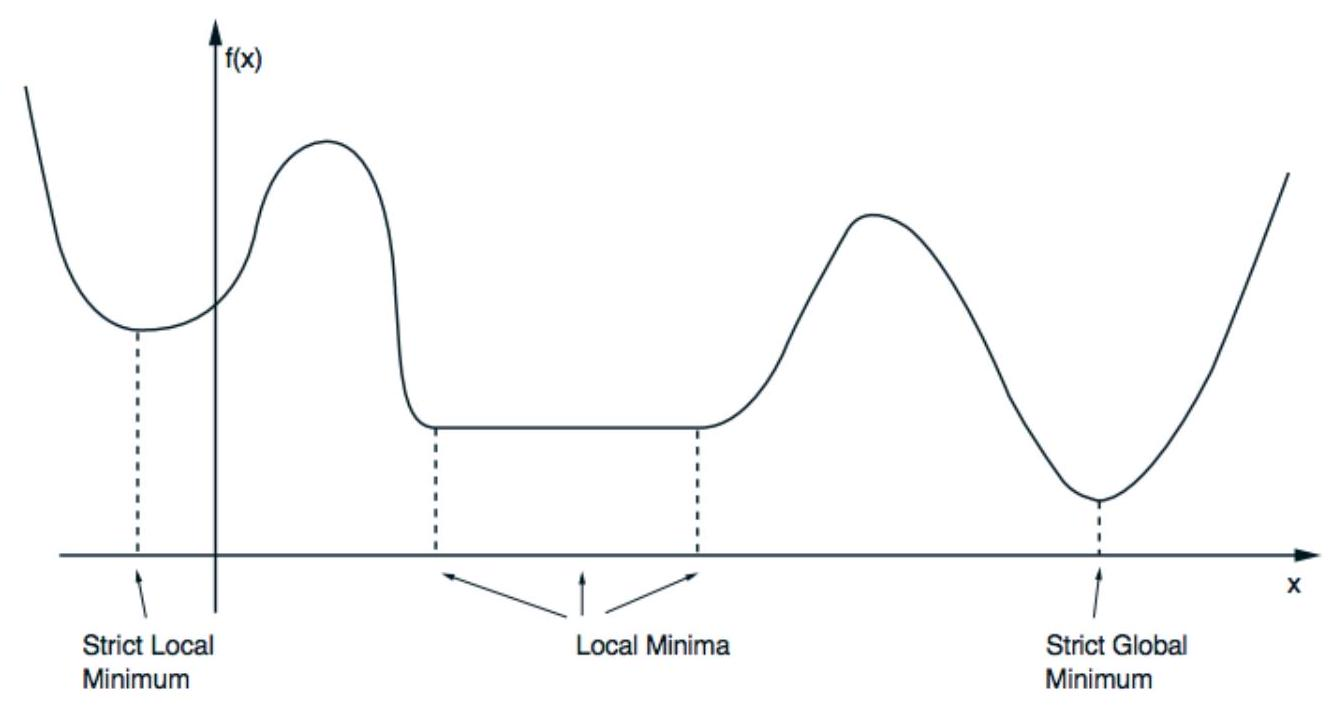
\includegraphics[max width=\textwidth]{2023_12_30_4ff132a3450066e65b4fg-04}
\end{center}

The above figure is taken from Bertsekas, Nonlinear programming.

A vector $\mathbf{w}^{\star}$ is a local minimum of $\mathcal{L}$

if it is no worse than its neighbors;

i.e. there exists an $\epsilon>0$ such that,

$\mathcal{L}\left(\mathbf{w}^{\star}\right) \leq \mathcal{L}(\mathbf{w}), \quad \forall \mathbf{w}$ with $\left\|\mathbf{w}-\mathbf{w}^{\star}\right\|<\epsilon$

A vector $\mathbf{w}^{\star}$ is a global minimum

of $\mathcal{L}$ if it is no worse than all others,

$$
\mathcal{L}\left(\mathbf{w}^{\star}\right) \leq \mathcal{L}(\mathbf{w}), \quad \forall \mathbf{w} \in \mathbb{R}^{D}
$$

A local or global minimum is said to be strict if the corresponding inequality is strict for $\mathbf{w} \neq \mathbf{w}^{\star}$.

\section*{Smooth Optimization}
\section*{Follow the Gradient}
A gradient (at a point) is the slope of the tangent to the function (at that point). It points to the direction of largest increase of the function.

For a 2-parameter model, $\operatorname{MSE}(\mathbf{w})$ and $\operatorname{MAE}(\mathbf{w})$ are shown below.

(We used $\mathbf{y}_{n} \approx w_{0}+w_{1} x_{n 1}$ with $\mathbf{y}^{\top}=[2,-1,1.5]$ and $\mathbf{x}^{\top}=[-1,1,-1]$ ).
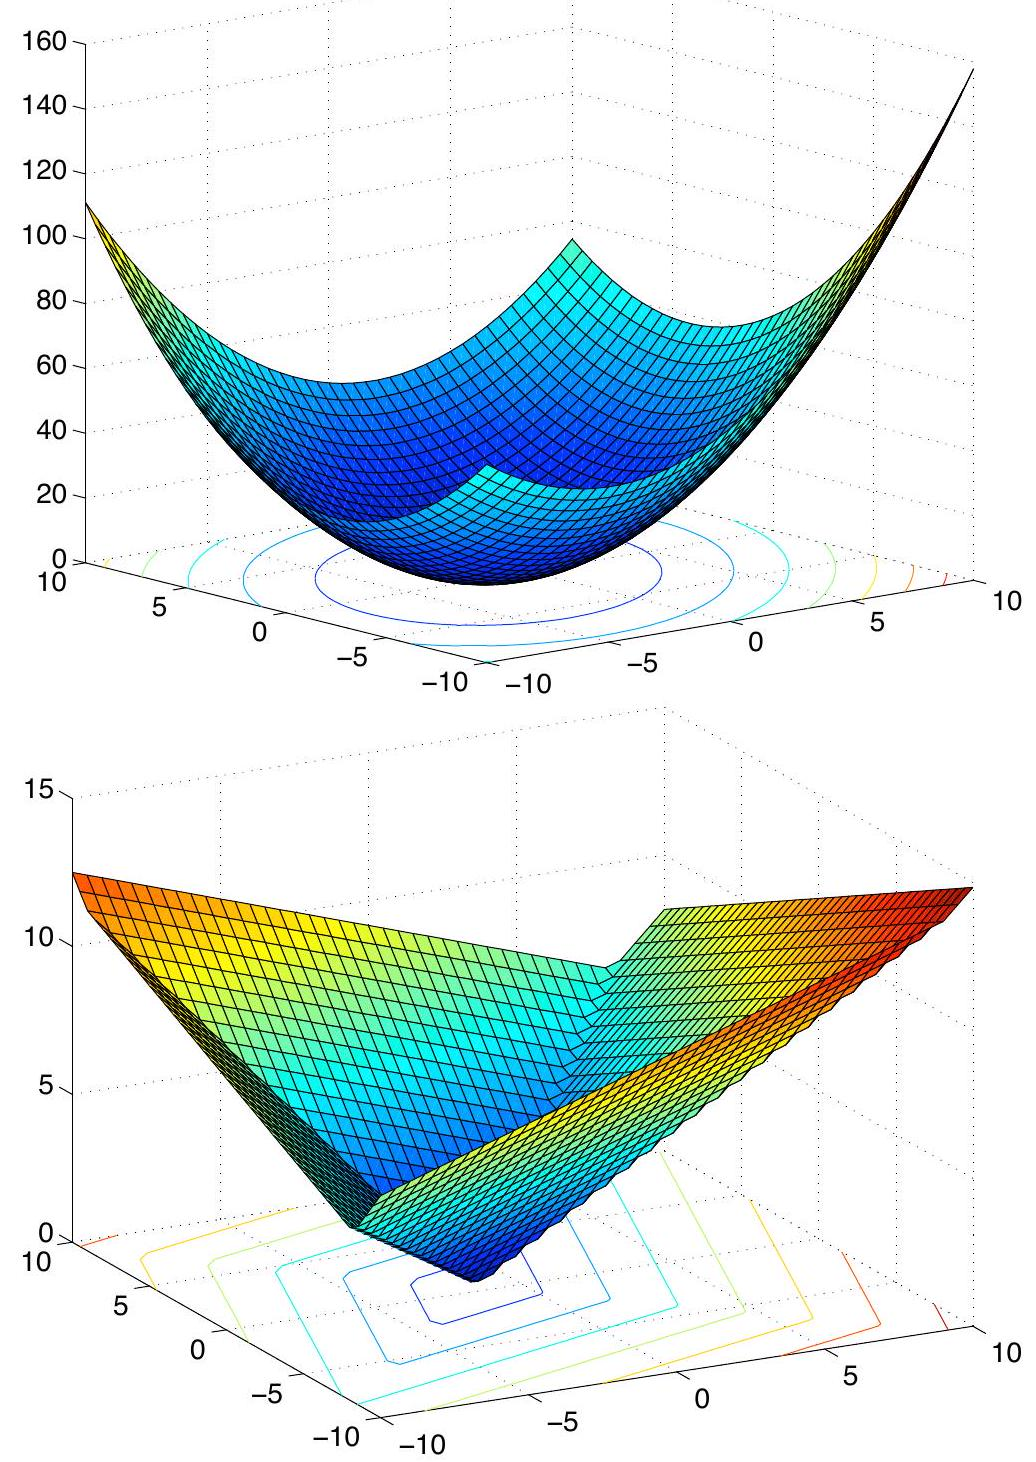
\includegraphics[max width=\textwidth, center]{2023_12_30_4ff132a3450066e65b4fg-05}

Definition of the gradient:

$\nabla \mathcal{L}(\mathbf{w}):=\left[\frac{\partial \mathcal{L}(\mathbf{w})}{\partial w_{1}}, \ldots, \frac{\partial \mathcal{L}(\mathbf{w})}{\partial w_{D}}\right]^{\top}$

This is a vector, $\nabla \mathcal{L}(\mathbf{w}) \in \mathbb{R}^{D}$.

\section*{Gradient Descent}
To minimize the function, we iteratively take a step in the (opposite) direction of the gradient

$$
\mathbf{w}^{(t+1)}:=\mathbf{w}^{(t)}-\gamma \nabla \mathcal{L}\left(\mathbf{w}^{(t)}\right)
$$

where $\gamma>0$ is the step-size (or learning rate). Then repeat with the next $t$.

Example: Gradient descent for 1parameter model to minimize MSE:

$$
w_{0}^{(t+1)}:=(1-\gamma) w_{0}^{(t)}+\gamma \bar{y}
$$

where $\bar{y}:=\sum_{n} y_{n} / N$. When is this sequence guaranteed to converge?

\section*{Gradient Descent for Linear MSE}
For linear regression

$\mathbf{y}=\left[\begin{array}{c}y_{1} \\ y_{2} \\ \vdots \\ y_{N}\end{array}\right], \mathbf{X}=\left[\begin{array}{cccc}x_{11} & x_{12} & \ldots & x_{1 D} \\ x_{21} & x_{22} & \ldots & x_{2 D} \\ \vdots & \vdots & \ddots & \vdots \\ x_{N 1} & x_{N 2} & \ldots & x_{N D}\end{array}\right]$

We define the error vector $\mathbf{e}$ :

$\mathrm{e}=\mathbf{y}-\mathbf{X w}$

and MSE as follows:

$$
\begin{aligned}
\mathcal{L}(\mathbf{w}) & :=\frac{1}{2 N} \sum_{n=1}^{N}\left(y_{n}-\mathbf{x}_{n}^{\top} \mathbf{w}\right)^{2} \\
& =\frac{1}{2 N} \mathbf{e}^{\top} \mathbf{e}
\end{aligned}
$$

then the gradient is given by

$\nabla \mathcal{L}(\mathbf{w})=-\frac{1}{N} \mathbf{X}^{\top} \mathbf{e}$

Computational cost. What is the complexity (\# operations) of computing the gradient?

a) starting from $\mathbf{w}$ and

b) given $\mathbf{e}$ and $\mathbf{w}$ ?

\section*{Variant with offset. Recall: Alter-}
native trick when also incorporating an offset term for the regression:

$\mathbf{y}=\left[\begin{array}{c}y_{1} \\ y_{2} \\ \vdots \\ y_{N}\end{array}\right] \quad \widetilde{\mathbf{X}}=\left[\begin{array}{ccccc}1 & x_{11} & x_{12} & \ldots & x_{1 D} \\ 1 & x_{21} & x_{22} & \ldots & x_{2 D} \\ \vdots & \vdots & \vdots & \ddots & \vdots \\ 1 & x_{N 1} & x_{N 2} & \ldots & x_{N D}\end{array}\right]$

\section*{Stochastic Gradient Descent}
Sum Objectives. In machine

learning, most cost functions are formulated as a sum over the training examples, that is

$$
\mathcal{L}(\mathbf{w})=\frac{1}{N} \sum_{n=1}^{N} \mathcal{L}_{n}(\mathbf{w})
$$

where $\mathcal{L}_{n}$ is the cost contributed by the $n$-th training example.

Q: What are the $\mathcal{L}_{n}$ for linear MSE?

\section*{The SGD Algorithm. The}
 stochastic gradient descent (SGD) algorithm is given by the following update rule, at step $t$ :$$
\mathbf{w}^{(t+1)}:=\mathbf{w}^{(t)}-\gamma \nabla \mathcal{L}_{n}\left(\mathbf{w}^{(t)}\right)
$$

\section*{Theoretical Motivation. Idea:}
Cheap but unbiased estimate of the gradient!

In expectation over the random choice of $n$, we have

$$
\mathbb{E}\left[\nabla \mathcal{L}_{n}(\mathbf{w})\right]=\nabla \mathcal{L}(\mathbf{w})
$$

which is the true gradient direction. (check!)

Mini-batch SGD. There is an intermediate version, using the update direction being

$$
\mathbf{g}:=\frac{1}{|B|} \sum_{n \in B} \nabla \mathcal{L}_{n}\left(\mathbf{w}^{(t)}\right)
$$

again with

$$
\mathbf{w}^{(t+1)}:=\mathbf{w}^{(t)}-\gamma \mathbf{g} .
$$

In the above gradient computation, we have randomly chosen a subset $B \subseteq[N]$ of the training examples. For each of these selected examples $n$, we compute the respective gradient $\nabla \mathcal{L}_{n}$, at the same current point $\mathbf{w}^{(t)}$.

The computation of $\mathbf{g}$ can be parallelized easily. This is how current deep-learning applications utilize GPUs (by running over $|B|$ threads in parallel).

Note that in the extreme case $B:=$ $[N]$, we obtain (batch) gradient descent, i.e. $\mathbf{g}=\nabla \mathcal{L}$.

\section*{SGD for Linear MSE}
See Exercise Sheet 2.

Computational cost. For linear MSE, what is the complexity (\# operations) of computing the stochastic gradient?

(using only $|B|=1$ data examples)

\section*{Non-Smooth Optimization}
An alternative characterization of convexity, for differentiable functions is given by

$\mathcal{L}(\mathbf{u}) \geq \mathcal{L}(\mathbf{w})+\nabla \mathcal{L}(\mathbf{w})^{\top}(\mathbf{u}-\mathbf{w}) \quad \forall \mathbf{u}, \mathbf{w}$

meaning that the function must always lie above its linearization.

\section*{Subgradients}
A vector $\mathbf{g} \in \mathbb{R}^{D}$ such that

$$
\mathcal{L}(\mathbf{u}) \geq \mathcal{L}(\mathbf{w})+\mathbf{g}^{\top}(\mathbf{u}-\mathbf{w}) \quad \forall \mathbf{u}
$$

is called a subgradient to the function $\mathcal{L}$ at $\mathbf{w}$.

This definition makes sense for objectives $\mathcal{L}$ which are not necessarily differentiable (and not even necessarily convex).

If $\mathcal{L}$ is convex and differentiable at $\mathbf{w}$, then the only subgradient at $\mathbf{w}$ is $\mathbf{g}=\nabla \mathcal{L}(\mathbf{w})$.

\section*{Subgradient Descent}
Identical to the gradient descent algorithm, but using a subgradient instead of gradient. Update rule

$$
\mathbf{w}^{(t+1)}:=\mathbf{w}^{(t)}-\gamma \mathbf{g}
$$

for $\mathbf{g}$ being a subgradient to $\mathcal{L}$ at the current iterate $\mathbf{w}^{(t)}$.

\section*{Example: Optimizing Linear MAE}
\begin{enumerate}
  \item Compute a subgradient of the absolute value function
\end{enumerate}

$h: \mathbb{R} \rightarrow \mathbb{R}, h(e):=|e|$.

\begin{enumerate}
  \setcounter{enumi}{1}
  \item Recall the definition of the mean absolute error:
\end{enumerate}

$\mathcal{L}(\mathbf{w})=\operatorname{MAE}(\mathbf{w}):=\frac{1}{N} \sum_{n=1}^{N}\left|y_{n}-f_{\mathbf{w}}\left(\mathbf{x}_{n}\right)\right|$

For linear regression, its (sub)gradient is easy to compute using the chain rule. Compute it!

See Exercise Sheet 2.

\section*{Stochastic Subgradient Descent}
Stochastic SubGradient Descent (still abbreviated SGD commonly).

Same, $\mathbf{g}$ being a subgradient to the randomly selected $\mathcal{L}_{n}$ at the current iterate $\mathbf{w}^{(t)}$.

Exercise: Compute the SGD update for linear MAE.

\section*{Variants of SGD}
\section*{SGD with Momentum}
pick a stochastic gradient $\mathbf{g}$

$$
\begin{aligned}
& \mathbf{m}^{(t+1)}:=\beta_{1} \mathbf{m}^{(t)}+\left(1-\beta_{1}\right) \mathbf{g} \quad \text { (momentum term) } \\
& \mathbf{w}^{(t+1)}:=\mathbf{w}^{(t)}-\gamma \mathbf{m}^{(t+1)}
\end{aligned}
$$

\begin{itemize}
  \item momentum from previous gradients (acceleration)
\end{itemize}

\section*{Adam}
pick a stochastic gradient $\mathbf{g}$

$$
\begin{aligned}
\mathbf{m}^{(t+1)} & :=\beta_{1} \mathbf{m}^{(t)}+\left(1-\beta_{1}\right) \mathbf{g} \\
\mathbf{v}_{i}^{(t+1)} & :=\beta_{2} \mathbf{v}_{i}^{(t)}+\left(1-\beta_{2}\right)\left(\mathbf{g}_{i}\right)^{2} \quad \forall i \quad \text { (2nomentum term) } \\
\mathbf{w}_{i}^{(t+1)} & :=\mathbf{w}_{i}^{(t)}-\frac{\gamma}{\sqrt{\mathbf{v}_{i}^{(t+1)}}} \mathbf{m}_{i}^{(t+1)} \quad \forall i
\end{aligned}
$$

\begin{itemize}
  \item faster forgetting of older weights
  \item is a momentum variant of Adagrad
  \item coordinate-wise adjusted learning rate
  \item strong performance in practice, e.g. for self-attention networks
\end{itemize}

\section*{SignSGD}
pick a stochastic gradient $\mathbf{g}$

$$
\mathbf{w}_{i}^{(t+1)}:=\mathbf{w}_{i}^{(t)}-\gamma \operatorname{sign}\left(\mathbf{g}_{i}\right)
$$

\begin{itemize}
  \item only use the sign (one bit) of each gradient entry $\rightarrow$ communication efficient for distributed training
  \item convergence issues
\end{itemize}

\section*{Constrained Optimization}
Sometimes, optimization problems come posed with additional constraints:

$\min _{\mathbf{w}} \mathcal{L}(\mathbf{w}), \quad$ subject to $\mathbf{w} \in \mathcal{C}$.

The set $\mathcal{C} \subset \mathbb{R}^{D}$ is called the constraint set.
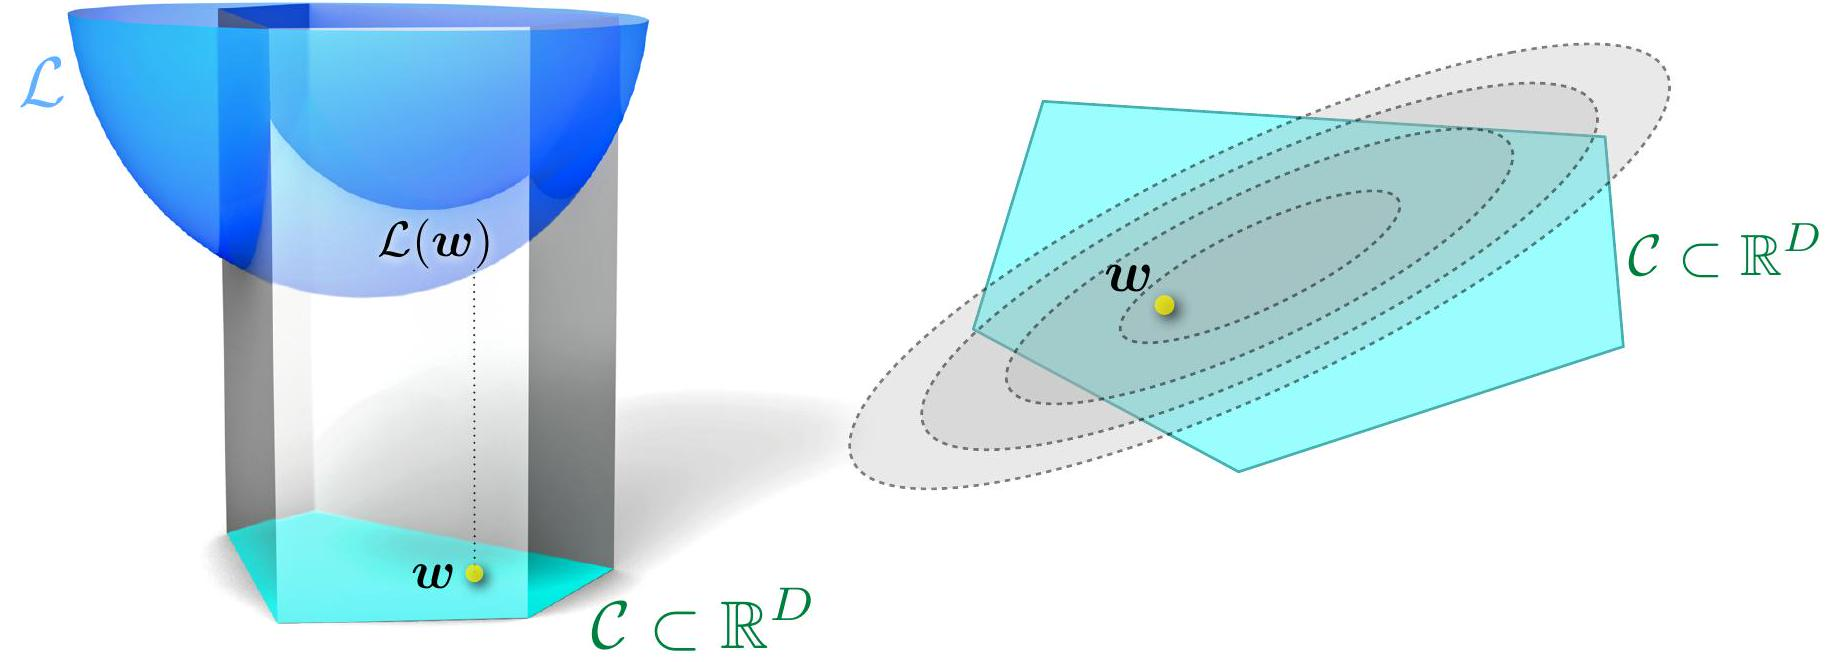
\includegraphics[max width=\textwidth, center]{2023_12_30_4ff132a3450066e65b4fg-15}

Solving Constrained Optimization Problems

A) Projected Gradient Descent

B) Transform it into an unconstrained problem

\section*{Convex Sets}
A set $\mathcal{C}$ is convex iff

the line segment between any two

points of $\mathcal{C}$ lies in $\mathcal{C}$, i.e., if for any

$\mathbf{u}, \mathbf{v} \in \mathcal{C}$ and any $\theta$ with $0 \leq \theta \leq 1$,

we have

$$
\theta \mathbf{u}+(1-\theta) \mathbf{v} \in \mathcal{C}
$$

\begin{center}
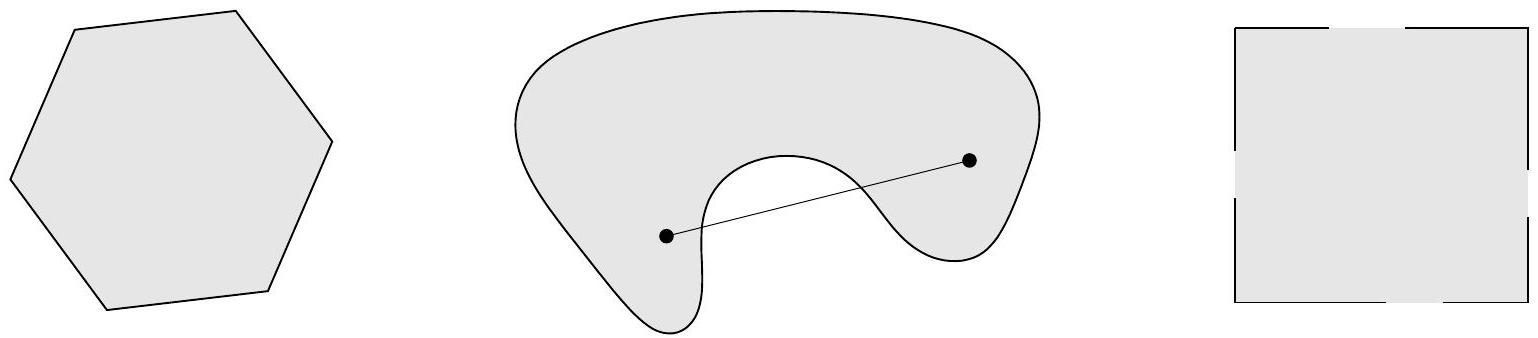
\includegraphics[max width=\textwidth]{2023_12_30_4ff132a3450066e65b4fg-16}
\end{center}

*Figure 2.2 from S. Boyd, L. Vandenberghe

\section*{Properties of Convex Sets}
\begin{itemize}
  \item Intersections of convex sets are convex
  \item Projections onto convex sets are unique.
\end{itemize}

(and often efficient to compute)

Formal definition:

$P_{\mathcal{C}}\left(\mathbf{w}^{\prime}\right):=\arg \min _{\mathbf{v} \in \mathcal{C}}\left\|\mathbf{v}-\mathbf{w}^{\prime}\right\|$.

\section*{Projected Gradient Descent}
Idea: add a projection onto $\mathcal{C}$ after every step:

$$
P_{\mathcal{C}}\left(\mathbf{w}^{\prime}\right):=\arg \min _{\mathbf{v} \in \mathcal{C}}\left\|\mathbf{v}-\mathbf{w}^{\prime}\right\| .
$$

Update rule:

$$
\mathbf{w}^{(t+1)}:=P_{\mathcal{C}}\left[\mathbf{w}^{(t)}-\gamma \nabla \mathcal{L}\left(\mathbf{w}^{(t)}\right)\right]
$$

\begin{center}
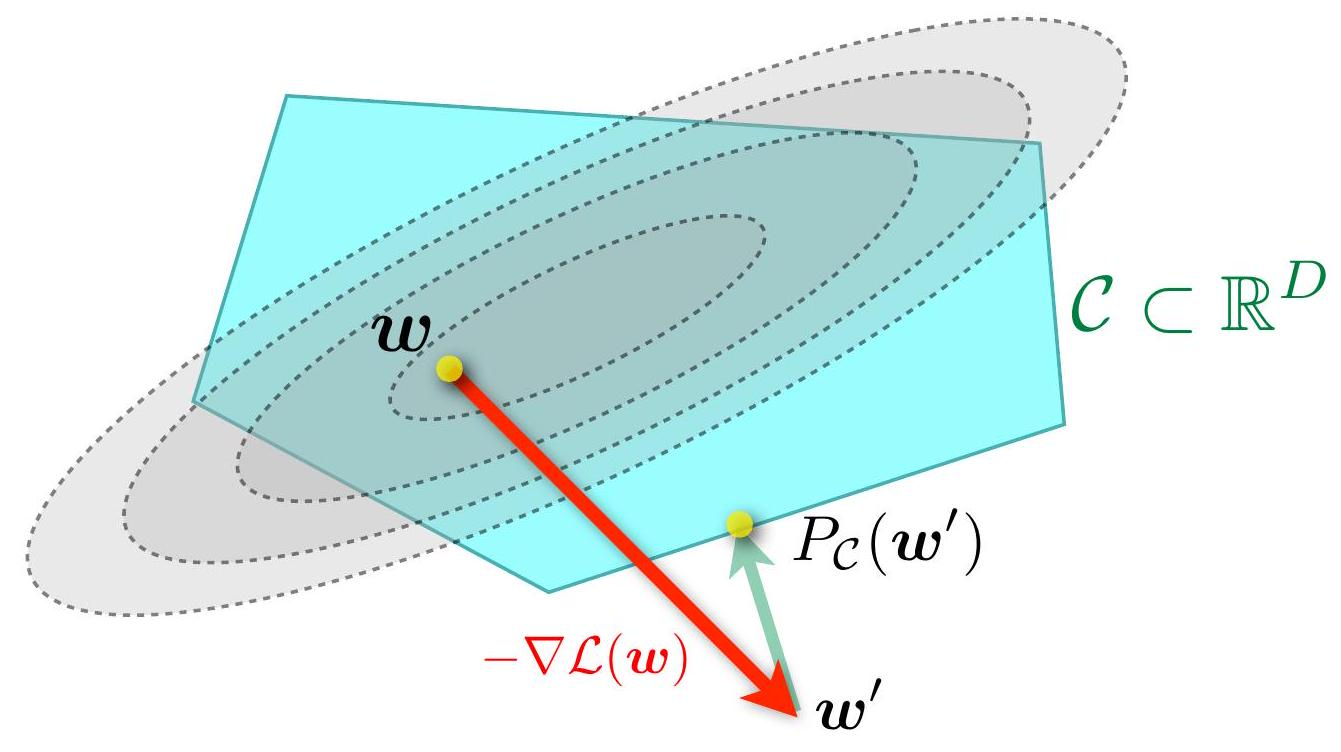
\includegraphics[max width=\textwidth]{2023_12_30_4ff132a3450066e65b4fg-17}
\end{center}

\section*{Projected SGD. Same SGD}
 step, followed by the projection step, as above. Same convergence properties.Computational cost of projection?

Crucial!

\section*{Turning Constrained into Unconstrained Problems}
(Alternatives to projected gradient

methods)

Use penalty functions instead of directly solving $\min _{\mathbf{w} \in \mathcal{C}} \mathcal{L}(\mathbf{w})$.

\begin{itemize}
  \item "brick wall" (indicator function)
\end{itemize}

$$
\begin{aligned}
& I_{\mathcal{C}}(\mathbf{w}):= \begin{cases}0 & \mathbf{w} \in \mathcal{C} \\
\infty & \mathbf{w} \notin \mathcal{C}\end{cases} \\
& \Rightarrow \min _{\mathbf{w} \in \mathbb{R}^{D}} \mathcal{L}(\mathbf{w})+I_{\mathcal{C}}(\mathbf{w})
\end{aligned}
$$

\begin{itemize}
  \item Penalize error. Example:
\end{itemize}

$$
\begin{aligned}
& \mathcal{C}=\left\{\mathbf{w} \in \mathbb{R}^{D} \mid A \mathbf{w}=\mathbf{b}\right\} \\
& \Rightarrow \min _{\mathbf{w} \in \mathbb{R}^{D}} \mathcal{L}(\mathbf{w})+\lambda\|A \mathbf{w}-\mathbf{b}\|^{2}
\end{aligned}
$$

\begin{itemize}
  \item Linearized Penalty Functions (see Lagrange Multipliers)
\end{itemize}

\section*{Implementation Issues}
For gradient methods:

\section*{Stopping criteria: When $\nabla \mathcal{L}(\mathbf{w})$}
is (close to) zero, we are (often) close to the optimum value.

Optimality: If the second-order derivative is positive (positive semidefinite to be precise), then it is a (possibly local) minimum. If the function is also convex, then this condition implies that we are at a global optimum. See the supplementary section on Optimality Conditions.

Step-size selection: If $\gamma$ is too big, the method might diverge. If it is too small, convergence is slow. Convergence to a local minimum is guaranteed only when $\gamma<\gamma_{\text {min }}$ where $\gamma_{\min }$ is a fixed constant that depends on the problem.

Line-search methods: For some objectives $\mathcal{L}$, we can set step-size automatically using a line-search method. More details on "backtracking" methods can be found in Chapter 1 of Bertsekas' book on "nonlinear programming".

\section*{Feature normalization and pre-}
 conditioning: Gradient descent is very sensitive to ill-conditioning. Therefore, it is typically advised to normalize your input features. In other words, we pre-condition the optimization problem. Without this, step-size selection is more difficult since different "directions" might converge at different speed.\section*{Non-Convex Optimization}
\begin{center}
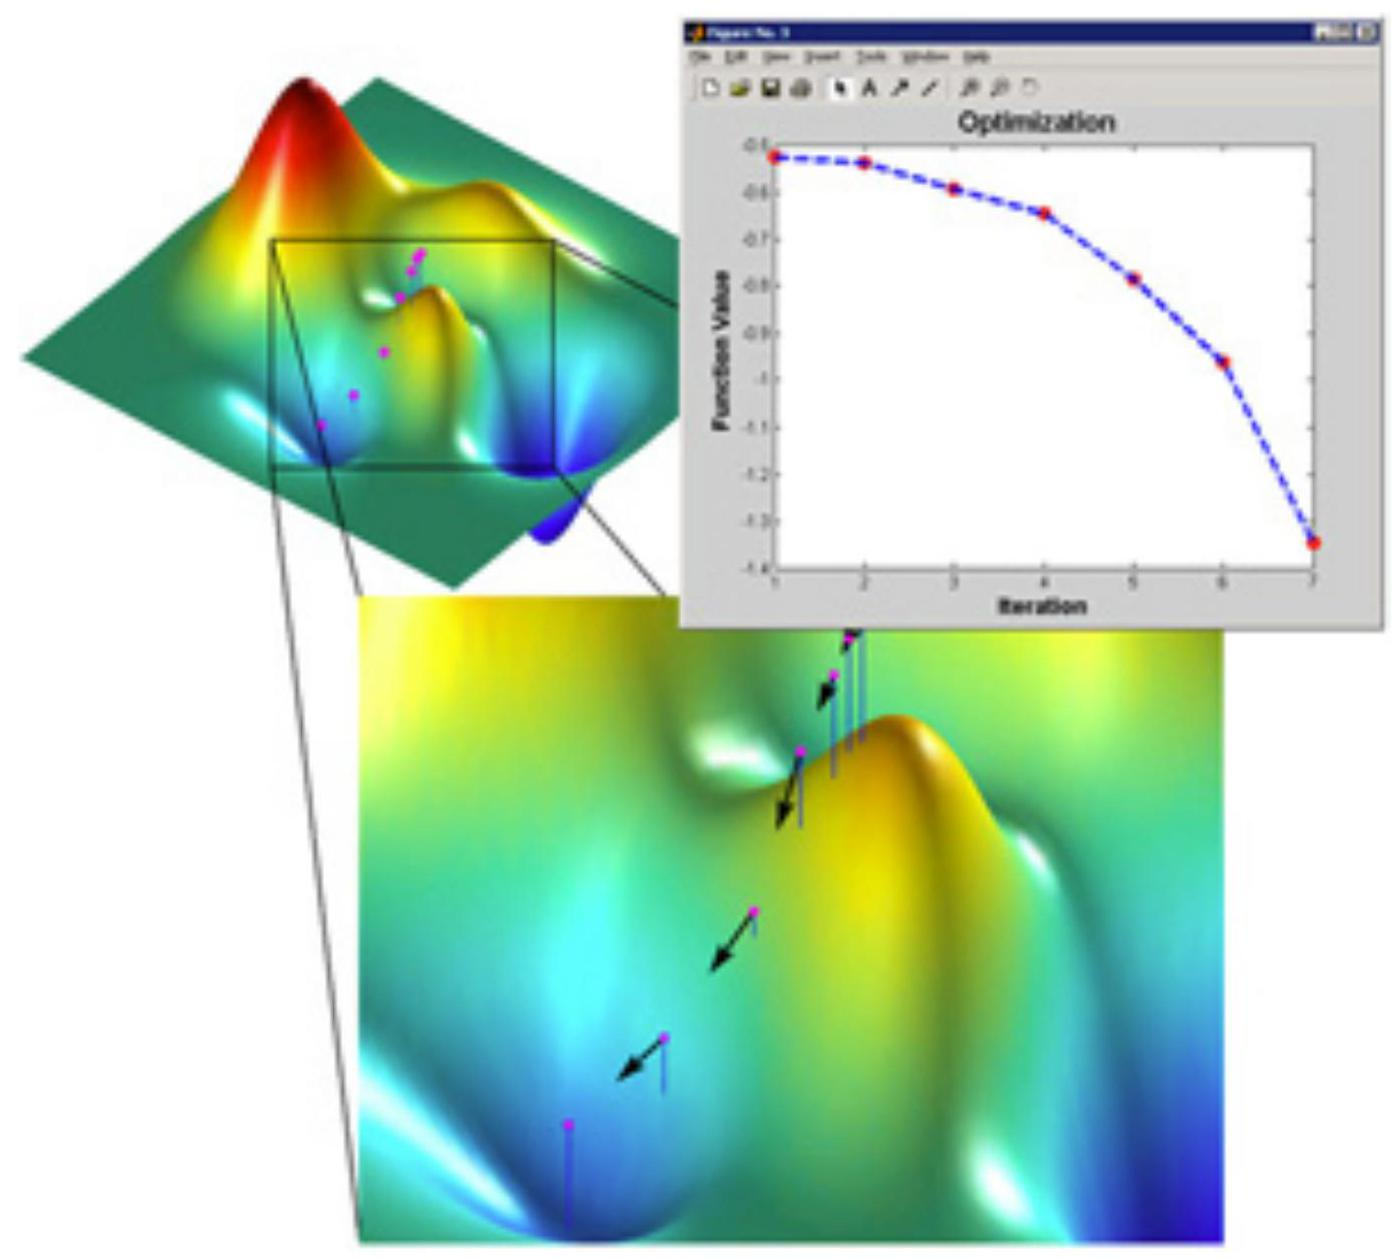
\includegraphics[max width=\textwidth]{2023_12_30_4ff132a3450066e65b4fg-21}
\end{center}

*image from \href{http://mathworks.com}{mathworks.com}

Real-world problems are not convex!

All we have learnt on algorithm design and performance of convex algorithms still helps us in the nonconvex world.

\section*{Additional Notes}
\section*{Grid Search and Hyper-Parameter Optimization}
Read more about grid search and other methods for "hyperparameter" setting:

\href{http://en.wikipedia.org/wiki/Hyperparameter_optimization#Grid_search}{en.wikipedia.org/wiki/Hyperparameter\_optimization\#Grid\_search}.

\section*{Computational Complexity}
The computation cost is expressed using the big- $\mathcal{O}$ notation. Here is a definition taken from Wikipedia. Let $f$ and $g$ be two functions defined on some subset of the real numbers. We write $f(x)=\mathcal{O}(g(x))$ as $x \rightarrow \infty$, if and only if there exists a positive real number $c$ and a real number $x_{0}$ such that $|f(x)| \leq c|g(x)|, \quad \forall x>x_{0}$.

Please read and learn more from this page in Wikipedia: \href{http://en.wikipedia.org/wiki/Computational_complexity_of_}{en.wikipedia.org/wiki/Computational\_complexity\_of\_} mathematical\_operations\#Matrix\_algebra .

\begin{itemize}
  \item What is the computational complexity of matrix multiplication?
  \item What is the computational complexity of matrix-vector multiplication?
\end{itemize}

\section*{Optimality Conditions}
For a smooth optimization problem, the first-order necessary condition says that at an optimum the gradient is equal to zero. Points of zero gradient are called critical points.

$$
\nabla \mathcal{L}\left(\mathbf{w}^{\star}\right)=\mathbf{0}
$$

We can use the second derivative to study if a candidate point is a local minimum (not a local maximum or saddle-point) using the Hessian
matrix, which is the matrix of second derivatives:

$$
\nabla^{2} \mathcal{L}(\mathbf{w}):=\frac{\partial^{2} \mathcal{L}}{\partial \mathbf{w} \partial \mathbf{w}^{\top}}(\mathbf{w})
$$

The second-order sufficient condition states that if

\begin{itemize}
  \item $\nabla \mathcal{L}(\mathbf{w})=\mathbf{0} \quad$ (critical point)
  \item and $\nabla^{2} \mathcal{L}(\mathbf{w}) \succ 0 \quad$ (positive definite),
\end{itemize}

then $\mathbf{w}$ is a local minimum.

The Hessian is also related to the convexity of a function: a twicedifferentiable function is convex if and only if the Hessian is positive semi-definite at all points.

\section*{SGD Theory}
As we have seen above, when $N$ is large, choosing a random training example $\left(\mathbf{x}_{n}, y_{n}\right)$ and taking an SGD step is advantageous:

$$
\mathbf{w}^{(t+1)}:=\mathbf{w}^{(t)}-\gamma^{(t)} \nabla \mathcal{L}_{n}\left(\mathbf{w}^{(t)}\right)
$$

For convergence, $\gamma^{(t)} \rightarrow 0$ "appropriately". One such condition called the Robbins-Monroe condition suggests to take $\gamma^{(t)}$ such that:

$$
\sum_{t=1}^{\infty} \gamma^{(t)}=\infty, \quad \sum_{t=1}^{\infty}\left(\gamma^{(t)}\right)^{2}<\infty
$$

One way to obtain such sequences is $\gamma^{(t)}:=1 /(t+1)^{r}$ where $r \in(0.5,1)$.

\section*{More Optimization Theory}
If you want, you can gain a deeper understanding of several optimization methods relevant for machine learning from this survey:

Convex Optimization: Algorithms and Complexity

\begin{itemize}
  \item by Sébastien Bubeck
\end{itemize}

And also from the book of Boyd \& Vandenberghe (both are free online PDFs)

\begin{center}
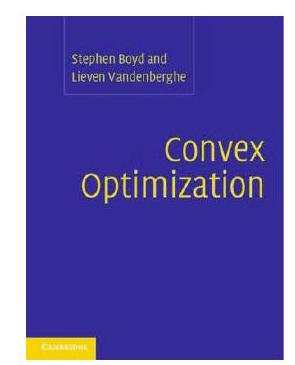
\includegraphics[max width=\textwidth]{2023_12_30_4ff132a3450066e65b4fg-24}
\end{center}

\section*{Exercises}
\begin{enumerate}
  \item Chain-rule
\end{enumerate}

\begin{center}

\includegraphics[max width=\textwidth]{2023_12_30_4ff132a3450066e65b4fg-24(1)}
\end{center}

If it has been a while, familiarize yourself with it again.

\begin{enumerate}
  \setcounter{enumi}{1}
  \item Revise computational complexity (also see the Wikipedia link in Page 6 of lecture notes).

  \item Derive the computational complexity of grid-search, gradient descent and stochastic gradient descent for linear MSE (\# steps and cost per step).

  \item Derive the gradients for the linear MSE and MAE cost functions.

  \item Implement gradient descent and gain experience in setting the step-size.

  \item Implement SGD and gain experience in setting the step-size.

\end{enumerate}

\end{document}